\documentclass[aps,prl,preprint,groupedaddress]{revtex4-1}
\usepackage{amssymb,amsfonts}
\usepackage[all,arc]{xy}
\usepackage{enumerate}
\usepackage{mathrsfs}

\usepackage{natbib}
\bibliographystyle{dinat}
\usepackage{graphicx}

\begin{document}
\title{GAIL and the Finch Song-Learning System}

\author{Artem Bolshakov}
\affiliation{Cornell University}

\date{\today}

\begin{abstract}
I'll compare Generative Adversarial Learning (GAIL) \cite{gail}, and some of the methods underlying this technique 
such as Generative Adversarial Networks and Inverse Reinforcement Learning, to the zebra finch neural system. 
Ultimately, I find that while GAIL is too specific a method to be a good analogy, 
Inverse Reinforcement Learning is a good analogy to the entire problem the finch faces 
(learning a task by imitating an expert in the present, for future reward), 
and it is possible that some specific brain regions act like the Discriminator in a Generative Adversarial Networ (GAN). 
I'll discuss directions to explore from here, 
as well as machine learning systems that might be inspired by elements of the finch neural architecture.
\end{abstract}

\maketitle

\section{Introduction}

While there are some superficial similarities, the GAIL algorithm and the finch system are fairly different. 
However, there are potential lessons for Machine Learning that can be teased out of the finch neural system; 
there are also some specific hypotheses that can be tested about whether or not finches use something like a GAN
in order to learn to imitate their tutor.

In order to discuss this, I will briefly review Reinforcement Learning, the finch system, 
and then Generative Adversarial Networks (with Generative Adversarial Imitation Learning as a special case), 
and then compare and contrast certain details of their function.

\section{Reinforcement Learning}

Briefly, let's review Reinforcement Learning, or RL, generally. 
This is a subset of AI in which an agent learns to perform actions that maximize reward in an environment. 

More precisely, it's a problem with a collection of states $S$, initial state $s_0 \in S$, 
actions $A$, a reward function $r(s, a)$, a transition function that measures the probability of being in $s'$ 
after action $a$ in state $s$ (written $p(s' | s, a)$ ), and a discount rate $\gamma$. 

Let's assume that, as a consequence of its previous actions, at timestep $t$ 
the agent finds itself in state $s_t$. 
The point of reinforcement learning is to find a policy, 
defined as the probability of action $a$ given state $s$ 
(written $\pi (a | s)$ )
that maximizes expected reward; 
that is, we want to choose an action $a$ such that 
$r_t + \gamma \overline{r_{t+1}} + \gamma^2 \overline{r_{t+2}} + \ldots$ 
(where $\overline{r_s}$ is the expected reward at timestep $s$) is as large as possible.

This is an important field in Machine Learning, but is also relevant to neurobiology. 
It is relevant specifically to the zebra finch in two ways. 

Most immediately, the finch learns to sing with the help of dopamine-modulated reinforcement signals. 
After a phrase which is perceived as good (or more precisely, better than expected), 
the synapses in Area X which just fired are made stronger, increasing the probability of repeating this behavior. 
I'll describe the neural circuitry of the zebra finch in more detail in the next section.

More fundamentally, however, singing is a behavior aimed at securing mates, or a behavior in pursuit of a reward. 
It's important to note that the finch usually does not experience this reward while it is learning, 
let alone have access to the female dopamine signals triggered by particular parts of the vocalization,
but it does have access to the vocalizations of mentors. 
From this point of view, learning to sing is similar to the problem of \emph{Inverse Reinforcement Learning}, or IRL; 
learning without access to the fundamental feedback function, but with access to the trajectories of experts. 
Specifically, IRL works by constructing a reward function $R$ under which the mentor actions are optimal; 
we can view the dopamine signals of the finch in this way.

I'll describe IRL in more detail in section $3$.

\section{The Zebra Finch System}

By imitiating a tutor, zebra finches learn a highly stereotyped song that they use later in life during courtship (see, for instance, \cite{nifmem}).
Finches have been used extensively as a model organism for the development of vocalization. 

The key neurological components of this system are illustreated in fig. \ref{fig1b} (Figure 1b from \cite{hvcchains}). 
I'll provide a brief overview of this system without going into detail 
about the experiments and history of how this understanding was developed over time; for that, I reccommend 
\cite{lman}, \cite{hvcchains}, \cite{dopamine}, \cite{jesseactorcritic}, \cite{nifmem}, or \cite{hvcmem}  among others.

The section of the brain which directly projects to the vocal muscles is known as RA (robust nucleus of the arcopallium). 
This section can be described as a "keyboard" for the rest of the system.

Two important brain regions project directly to RA: the HVC pre-motor nucleus (high vocal center), and 
LMAN (lateral magnocellular nucleus of the anterior nidopallium). 
HVC contains neurons that project both to RA and to other HVC neurons, forming "timing chains" where a neuron will 
trigger the correct "keys to play" in RA, then trigger the neurons corresponding to the next time-step. 
While projections from auditory regions have been hypthesized to play a role (See Fig $3$ in \cite{hvcchains}), 
the formation of these chains can largely be explained through Hebbian learning with some modifications (see \cite{hvcchains}), 
where the shorter-term changes in RA firing comes not from HVC, but from LMAN 
(and the HVC projections to RA are strengthened through repetition).

While HVC serves to memorize the entie song sequence, LMAN seems to play a more immediate role in learning. 
First of all, it serves as a source of train-time variability, allowing the finch to try out different actions 
(lesioning LMAN creates a highly stereotyped vocalization, \cite{lman}). 
However, thanks to the effect of Area X (which receives timing information from HVC), LMAN actually sends a BIASED noise signal.

Shorter-term learning, then, is in the projections from Area X to LMAN. 
These are trained through dopamine-mediated reinforcement learning, 
where any connections that fired shortly before a dopamine spike are strengthened, 
while any connections that fired shortly before a relative lack of dopamine 
(a dopamine signal below the basline rate) are weakened (see \cite{dopamine}).

The structure of the dopamine signal itself, then, determines what the finch learns. 
The dopaminergic connection comes from an area known as VTA (ventral tegmental area). 
This area in turn recieves signals from AIV (ventral intermediate arcopallium) and vBG (ventral Basal Ganglia) (see \cite{jesseactorcritic} for more details). 
AIV seems to encode the "true" error, or the difference between the performance and the tutor, 
while vBG predicts the AIV signal and compensates for it - in effect, serving as a "prediction error." 
That way, any improvement in performance is rewarded by VTA (produces a dopamine spike). 
The AIV, vBG, and VTA system serves as the "critic" in a classic actor-critic motif \cite{jesseactorcritic}.

To summarize, the zebra finch system seems to be a classic actor-critic motif, 
with AIV, vBG and VTA serving as the critic, while Area X, LMAN, HVC and RA are the "actor." 
AIV records true error, vBG adjusts that error based on expected performance, and all of this information is integrated by VTA. 
The dopaminergic signal is used to adjust Area X in order to improve song performance.

From another side, we know from behavioral studies that finches learn to imitate their tutors. 
How does information from tutor vocalizations ultimately affect this entire process? 
To the best of my understanding, this process is not well-understood 
(although HVC, motor circuits, and a brain region known as NIf (pallial sensorimotor nucleus interfacialis of the nidopallium) 
seems to play a role \cite{nifmem}, \cite{hvcmem}).
but I hope to look at some hypotheses on the subject based on Inverse Reinforcement Learning advances in Machine Learning, 
and in Generative Adversarial Imitation Learning, or GAIL, specifically.

\begin{figure}[h]
   \centering
   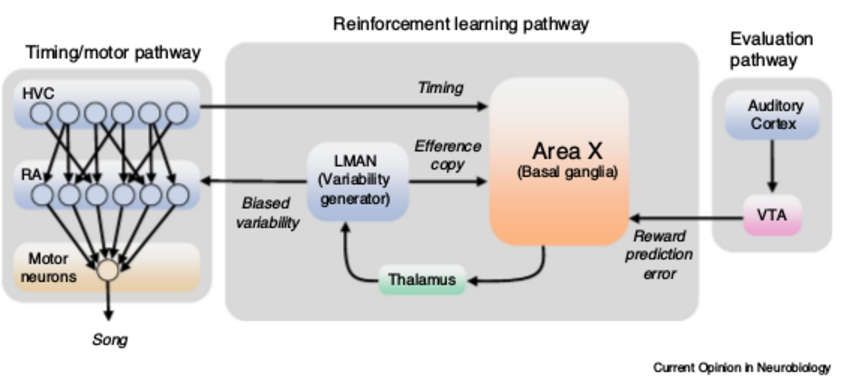
\includegraphics[width=1.0\textwidth]{jqfigs/HVC_fig1b.pdf}
   \caption{\label{fig1b} Figure 1b from \cite{hvcchains}, showing the basic structure of the zebra finch song learning and performance circuitry.}
\end{figure}
%[FIG 1b]


\section{GAIL}

\subsection{GANs}

Given data $x$ obeying $x ~ P(x)$ ($P$ is the probability distribution from which $x$ is drawn), 
a common problem of unsupervised machine learning is approximating 
the underlying probability distribution $P$ with $\widetilde{P}$. 
There are several uses for this, such as anomaly detection, making predictions about future examples, 
and especially drawing new samples $y$ from the modeled distribution $\widetilde{P}$.

Many techniques exist for computing $\widetilde{P}$ from data, both classical, such as Gaussian Mixture Models, 
and deep, such as a multide of variations on autoencoders and variational autoencoders. 
One method that has become particularly important for high-dimensional data, especially images, 
is Generative Adversarial Networks, or GANs, introduced in $2014$ in \cite{gan}.

There are two primary components to a GAN, each optimizing a different loss function: the Generator and the Discriminator. 
The Generator takes random input $z$ 
(usually multivariate Gaussian noise), and produces $G(z)$ with the same dimensionality as the input data. 
The Discriminator, meanwhile, takes as input $x$ with the dimensionality of the data, 
and tries to determine whether it is looking at real or simulated data. 
There are many different exact forms that this loss can take, 
but one of the more common ones essentially has the Discriminator output a number $D(x)$ 
interpreted as the probability of the sample, 
with the Discriminator loss trying to maximize $\log (D(x)) + \log (1 - D(G(z)))$,
while the generator tries to maximize $\log (D(G(z))$ for simulated data (see section $3$ in \cite{gan}).

In almost all realizations, both are trained simultaneously, 
although it is sometimes advised to train $D$ to its optimal performance before letting $G$ improve, 
ithen retraining $D$, in stages. 
Regardless of the exact dynamics, however, it is important to note that both improve together; 
one is not trained and frozen, the way the finch's system appears to be.

\subsection{IRL and GAIL}

Inverse Reinforcement Learning (IRL) is a technique that learns to imitate an expert by attempting to design a cost function 
$c(s, a)$ which the expert must be optimizing \cite{gail}.
The inventors of GAIL claim that this method often doesn't scale to complex environments, 
where a trajectory collection of reasonable size can't possibly provide enough information 
to evaluate the cost $c(s, a)$ (the cost of action $a$ in state $s$) everywhere. 
Furthermore, they derive that the problem of both deriving and then using such a cost 
is fundamentally equivalent to trying to find a policy $\pi$ whose 
trajectories occupy the same states $s$ and actions $a$ as the expert policy, 
and that taking this approach directly (matching occupancies) 
is a faster algorithm useful for larger reinforcement learning problems.

The basic structure of the GAIL algorithm is in figure \ref{GAILalgo}, copied here from page $7$ in \cite{gail}. 
Fundamentally, the structure is very similar to any other GAN.

In the first step, we use the existing policy $\pi_{\theta_i}$ 
and the expert policy $\pi_E$ to sample trajectory sets $\tau_E$ and $\tau_i$. 
We then use both sets of trajectories to update 
the discriminator $D(s, a)$, which provides a measure about whether a state-action pair $(s, a)$ is more 
expert-like or trainee-like. 

\begin{figure}[h]
   \centering
   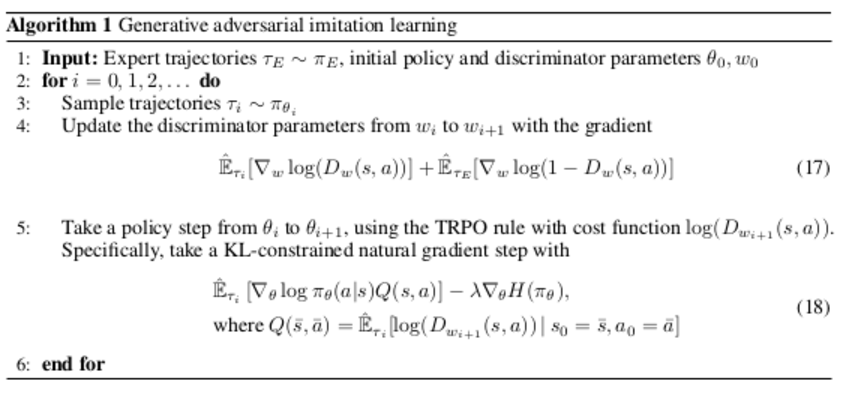
\includegraphics[width=1.0\textwidth]{jqfigs/GAILalgo.pdf}
   \caption{\label{GAILalgo} GAIL algorithm, from \cite{gail}}
\end{figure}

In the second step, then, the signal from the Discriminator is used to update the policy generating parameters
$\theta$. There are three uances here. 

The first is the entropy term $H$, encouraging policies that are not just repetitions of expert trajectories; 
but this is relatively unimportant when comparing to the finch.
The second is that the policy parameters $\theta$ 
(unlike the Discriminator parameters $w$) 
are updated not using the traditional gradient descent algorithm Adam, but instead TRPO 
(Trust Region Policy Optimization; see \cite{trpo}),
which makes certain that the new policy isn't too different from the old technique 
(measured in KL divergence over the probability of being in a particular system state).

Finally (and most importantly), it needs to be undestood that the $Q$ signal is a little more sophisticated than 
the Discriminator signal $D$ itself; 
rather, it is the empirically averaged value of $\log D$ over all trajectories that start 
in the given pair $(\tilde s, \tilde a)$ (this is at the end of the textbox \ref{GAILalgo}). 
In this way, $Q(s, a)$ is dependent on the "futures" of previous trajectories that started in $(\tilde s, \tilde a)$. 
From the best of my understanding, this is what gives this method power - the Discriminator is very simple, 
looking only at the state and the action in a given moment, but this gives a rich signal to the policy, 
which evaluates its performance based on how closely the "futures" it creates follow the "futures" created by the expert.

\section{Discussion}

We can now return to the question, how relevant are Inverse RL and GAIL to the finch system?

To start off, the finch is clearly solvng an inverse RL problem:
trying to learn a behavior (singing) to maximize a reward (mating) 
from expert examples (mentors) without access to the underlying reward function at train time.

However, it's also evident that the available traces are a little different than those available for GAIL. 
Specifically, GAIL works with traces that contain both the expert state sequences 
$\{ s_i \}$ and the action sequences $\{ a_i \}$. 
However, in the most straightforward translation from ML theory to the finch system, 
the audio profile at a given time $t$ is the state $s_t$, 
while the action $a_t$ is best interpreted as the muscle activation at a given time. 
From this point of view, it's clear that the finch only has access to the state sequence, not the action sequence. 
In fact, the problem of learning a difficult sequence of vocalizations 
boils down to learning a fast sequence of muscle activations from trial and error; 
learning the action sequence from the state sequence is the entire point. 
Of course, it's still possible to imagine an algorithm that learns from expert state-traces alone, 
but that would be an entirely different algorithm. 

It is also worth noting that GAIL is a very specific algorithm, 
and uses the discriminator signal summed over all "futures" of a state-action pair (the $Q$ function). 
The finch seems to only have a signal that is local in time, 
computing how similar \emph{the current syllable} is to the syllable the tutor pronounced at this point in the song.

In short, while analogies can be drawn to IRL, Discriminators, and other algorithms, 
without a deep understanding of how exactly AIV and other auditory circuits are trained, 
it's not quite possible to set up simple experiments to determine which one is closest to finch behavior.

\subsection{Comparing With the Classic GAN framework}

In GAIL, like most GANs, the Discriminator is trained alongside the Generator. 
It's worth noting here that \cite{hvcmem}
emphasizes how periods of vocal activity are interleaved with episodes of tutuoring for young finches. 
On the other hand, the finch continues to train singing long after no longer being exposed to the tutor. 
It would be very worthwhile to understand how AIV changes between tutoring episodes in young finches, 
and try to fully understand the difference between birds that have a single exposure to the tutor 
with those that have access to multiple tutoring sessions.

\subsection{AIV Development Directions}

It's possible that some algorithm - whether IRL or something related - will be a good analogy once we learn more. 
However, at the moment, probably the most interesting thing to understand is how the "true" error signal (from the AIV) is trained, 
using both behavioral and neurological studies. 

For instance, it would be interesting to know whether hearing one's own vocalizations changes the error signal, 
for instance as a "negativ example."
Specifically, if the finch has a small but consistent "error" in its song, does the AIV error signal become better at picking it up over time 
(even as the VTA learns to expect and ignore the error)? 
If so, we really do have a "discriminator" on our hands, learning to tell the difference between the finch's own performance and the tutor's 
(even if the algorithm doesn't match GAIL entirely). 
If not, supervised learning really remains the best analogy.

It would be very significant if the vocal error signal (or some precursor) can be computed during passive listening, not just during practice. 
For instance, it would be possible to see whether there was any innateness to this signal, 
and whether this signal could predict tutor selection (or tutor switching) behaviors. 

FInally, its worth noting that all of the algorithms mentioned above are stochastic, 
and can encode policies with many different paths through the state space just as well as policies with just one path. 
Therefore, everything that was mentioned about finches applies equally well to other songbirds with variable songs. 
It would be fascinating to understand exactly why finches only learn one variation while many other birds learn multiples. 
Possibly, this has more to do with the structure of the "actor" - HVC, Area X, LMAN - 
but it might be a consequence of the reward structure, too.

All of this is speculation by a non-neuroscientist, of course, but the takeaway is this: 
\emph{in order to determine which algorirthm the finch uses to learn from the mentor, 
we need to understand the neurobiology behind how this signal was learned.}

\subsection{Ideas for ML}

I think that it is easier to go in the other direction: finding inspiration for GANs and other generative models from the finch system. 

For instance, the feeback signal in GANs is, for lack of a better word, far less \emph{specific} than in the finch. 
The finch has a signal that is specific to the time when the syllable was pronounced, as well as an 
Actor-Critic framework that allows for incremental advances, even if the finch is already good at some syllables but struggling with others.

In GANs, however, there is only one number for an entire complex output, like an image. 
In theory, the gradient of this number with respect to the parameters $\theta_G$ of the generator $G$ 
should allow for improvement regardless, but in practice, \emph{mode collapse}, 
where the generator learns to reproduce only a limited portion of the sample distribution, is a very common problem. 

In the finch, the AIV delivers not just a signal about how well each vocalization matched the distribution of mentor vocalizations, 
but also whether or not the vocalization matches the \emph{type of vocalization that comes at time $t$ in the song.} 
Wouldn't it be great if we had some additional variable to replace time for the GAN? 
That is, wouldn't it be great if we could ask not just "how likely is it that this image came from ImageNet," 
but instead "how likely is it that this image is corresponds to the coordinate $z$ in the distribution of ImageNet images?" 
And there is, in fact, a great technique that does precisely that, known as a VAE-GAN \cite{vaegan}, from 2015. 

It's also possible that a fruitful direction is including the actor-critic framework in GANs, 
in order to learn all parts of a distribution;
fig. \ref{ActorCriticGAN} describes such a method augmenting the VAE-GAN, for instance. 
I also believe that neuromorphic systems for generating data can translate almost 
one-for-one the finch actor-critic architecture into ML.

\begin{figure}[h]
   \centering
   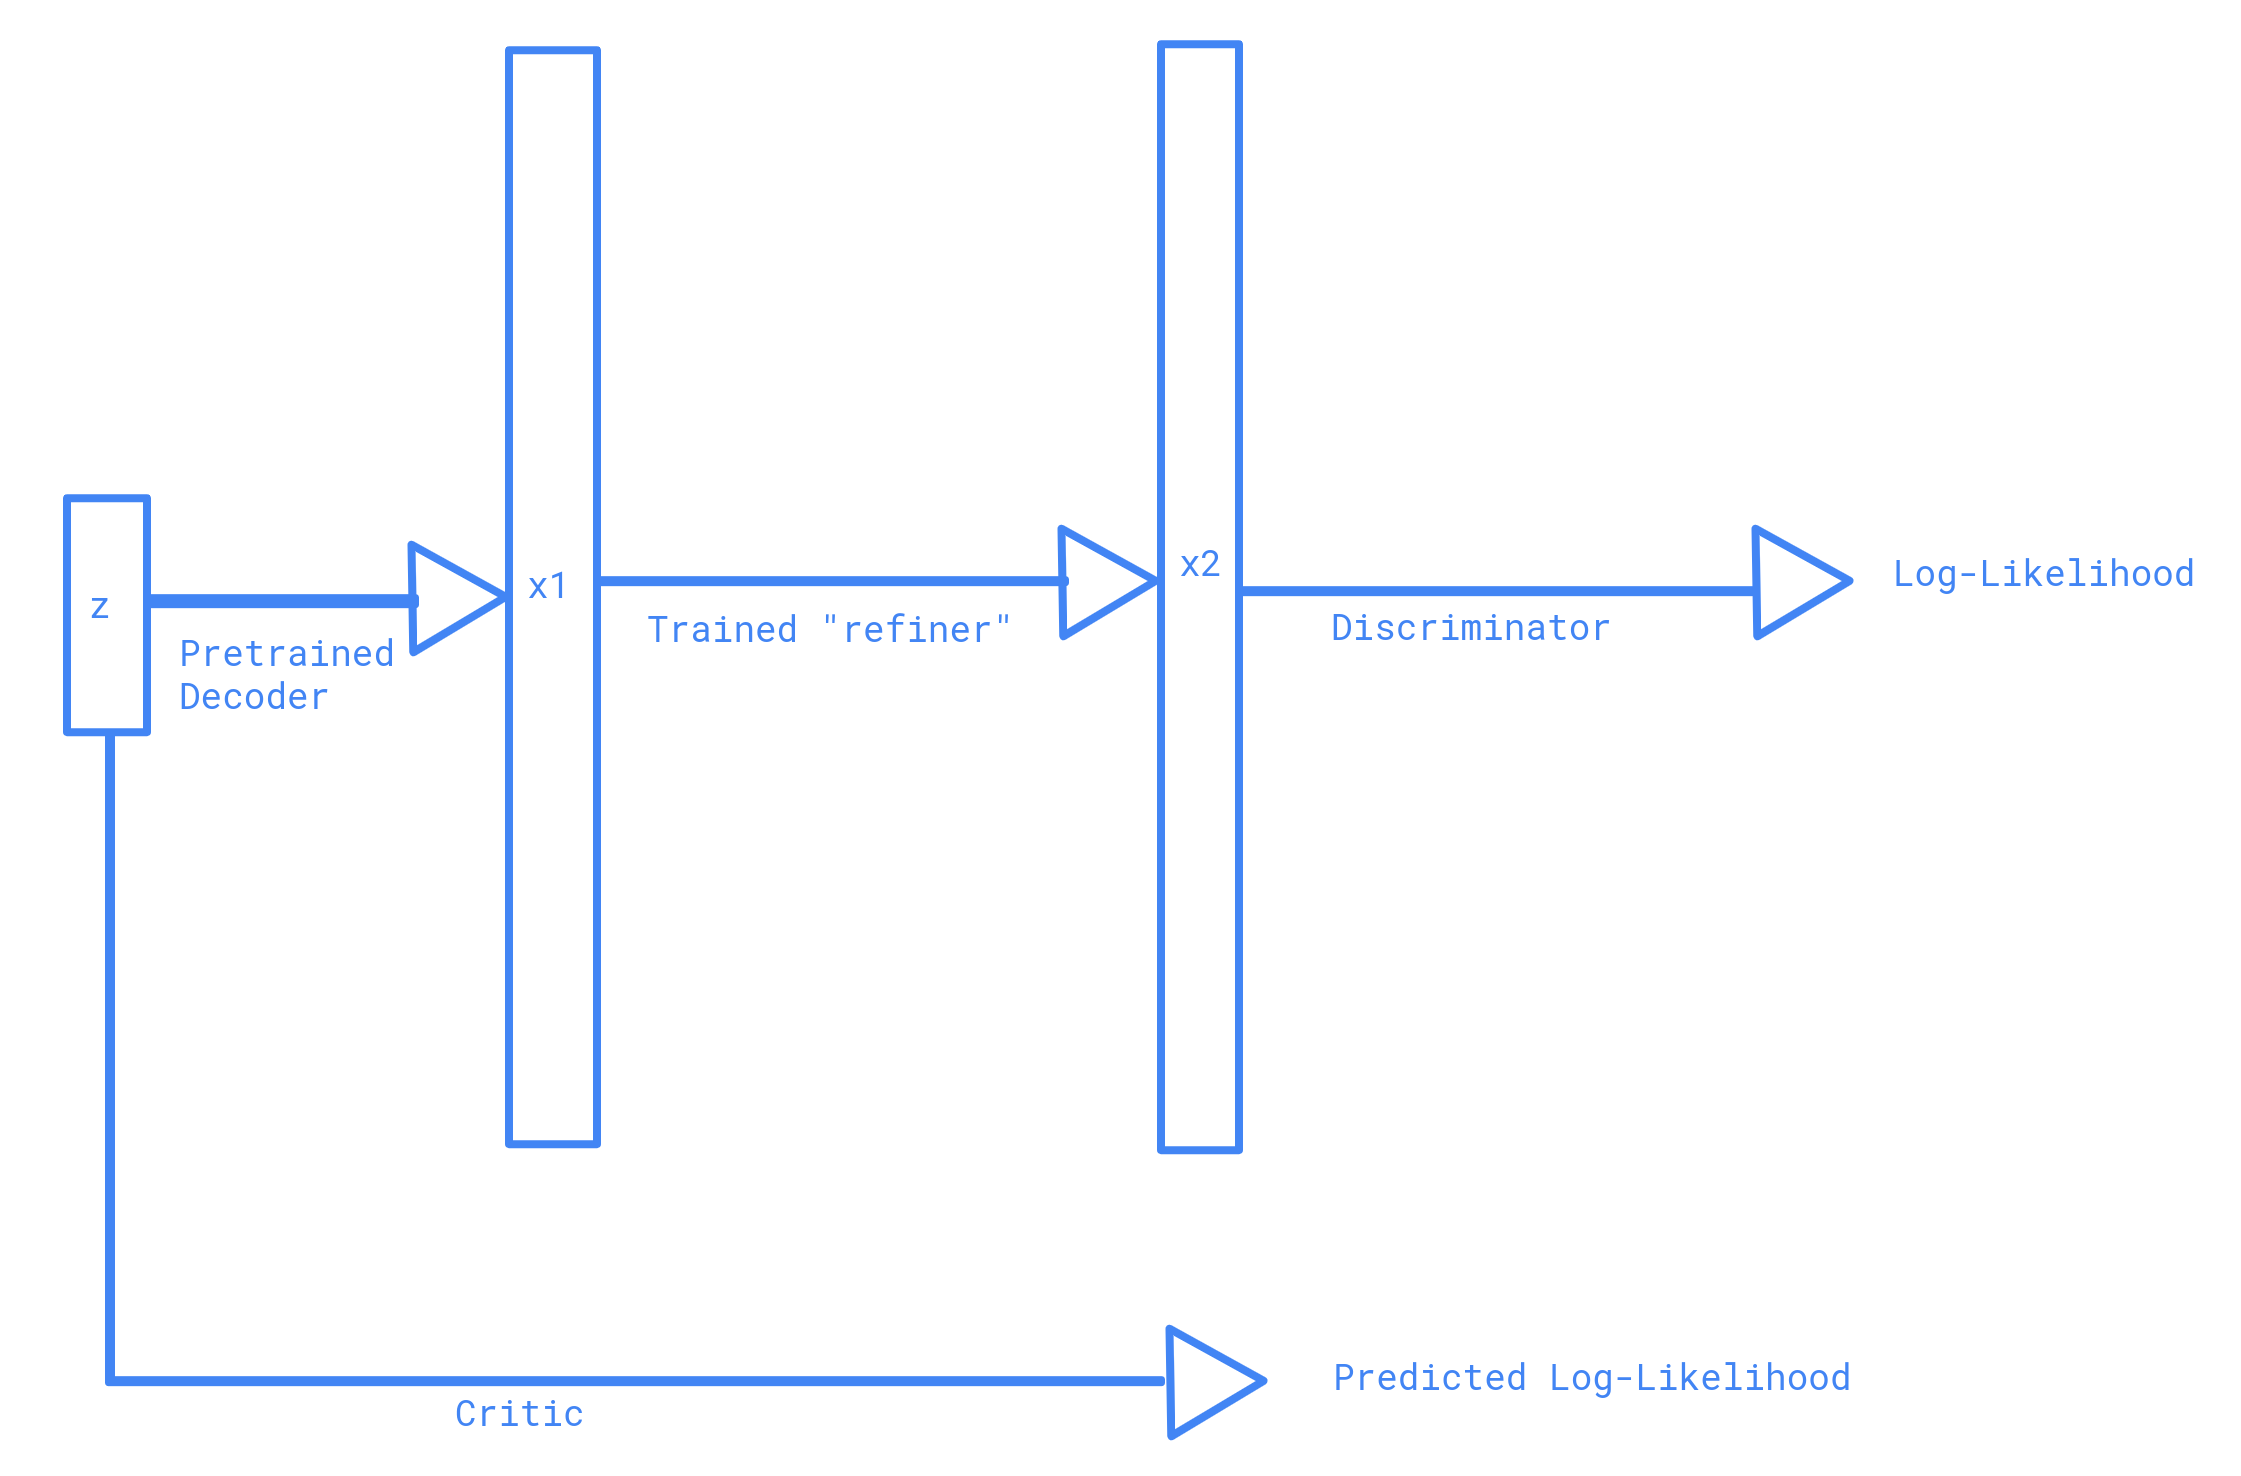
\includegraphics[width=1.0\textwidth]{jqfigs/ActorCriticGAN.png}
   \caption{\label{ActorCriticGAN} VAE GAN with an additional actor-critic structure. A slowly-trained critic can be used to focus training on difficult types of images.}
\end{figure}

\clearpage
\bibliography{jesseq}{}

\clearpage
\widetext
\end{document}

